% Author: Izaak Neutelings (Februari, 2020)

\documentclass[border=3pt,tikz]{standalone}
\usepackage{amsmath} % for \dfrac
\usepackage{physics,siunitx}
\usepackage{tikz,pgfplots}
\usetikzlibrary{angles,quotes} % for pic (angle labels)
\usetikzlibrary{decorations.markings}
\tikzset{>=latex} % for LaTeX arrow head
\usepackage{xcolor}
\colorlet{Rcol}{green!60!black}
\colorlet{myblue}{blue!70!black}
\colorlet{myred}{red!70!black}
\colorlet{Ecol}{orange!90!black}
\tikzstyle{Rline}=[Rcol,thick]
\tikzstyle{gline}=[Rcol,thick]
\tikzstyle{bline}=[myblue,thick]
\tikzstyle{rline}=[myred,thick]
\def\xmax{4.0}
\def\ymax{2.2}
\def\tick#1#2{\draw[thick] (#1) ++ (#2:0.03*\ymax) --++ (#2-180:0.06*\ymax)}
\newcommand\EMF{\mathcal{E}} %\varepsilon}


\begin{document}


% MAGNETIZATION vs. Bext
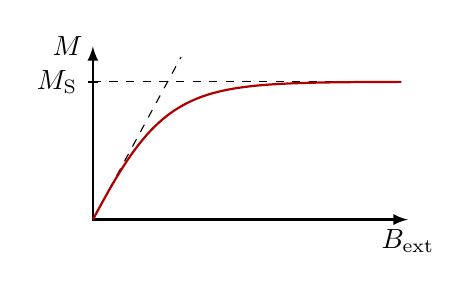
\begin{tikzpicture}
  \def\a{1.75} % amplitude
  \def\c{0.90}
  \def\t{1.00} % slope
  \coordinate (O) at (0,0);
  \coordinate (X) at (\xmax,0);
  \coordinate (Y) at (0,\ymax);
  \coordinate (Q) at (0,\a);
  \coordinate (T) at (\t,\a);
  \coordinate (Tx) at (\t,0);
  
  % AXIS
  \draw[<->,thick]
    (X) node[below] {$B_\text{ext}$} -- (O) -- (Y) node[left] {$M$};
  \tick{Q}{0} node[left] {$M_\mathrm{S}$}; 
  %\tick{Tx}{90} node[below] {$\tau = RC$};
  
  % PLOT
  \draw[dashed] (Q) --++ (0.98*\xmax,0);
  %\draw[dashed] (Tx) -- (T);
  %\draw[dashed] (O) -- (T);
  \draw[dashed,samples=100,smooth,variable=\x,domain=0:0.28*\xmax]
    plot(\x,{\a*\t*\x/sqrt(\c))});
  \draw[rline,samples=100,smooth,variable=\x,domain=0:0.98*\xmax]
    plot(\x,{\a*sinh(\t*\x)/sqrt(sinh(\t*\x)^2+\c)});
  
\end{tikzpicture}


% MAGNETIZATION vs. kT
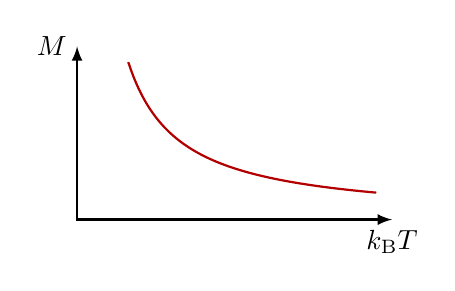
\begin{tikzpicture}
  \def\a{1.3}
  \coordinate (O) at (0,0);
  \coordinate (X) at (\xmax,0);
  \coordinate (Y) at (0,\ymax);
  
  % AXIS
  \draw[<->,thick]
    (X) node[below] {$k_\mathrm{B}T$} -- (O) -- (Y) node[left] {$M$};
  
  % PLOT
  \draw[rline,samples=100,smooth,variable=\x,domain={1.1*\a/\ymax}:0.95*\xmax]
    plot(\x,\a/\x);
  %\node[above right] at (1.4,1.8) {$E \sim \dfrac{1}{T}$};
  
\end{tikzpicture}


\end{document}
